\begin{frame}
	\frametitle{Klimamodelle und Restbudget - Zusammenfassung}

	\begin{columns}
    \column{0.3\linewidth}
      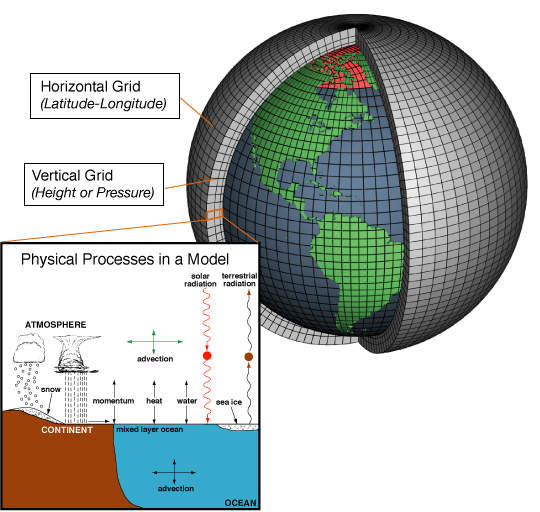
\includegraphics[width=0.9\linewidth]{bilder/AtmosphericModelSchematic.png}
    \column{0.7\linewidth}
      \begin{itemize}
        \item Klimamodelle versuchen die Erde ganzheitlich zu erfassen.
        \item Die Modelle sind sehr komplex, können aber nie alles abbilden.
        \begin{itemize}
          \item So viel wie nötig, so wenig wie möglich
          \item Modelle verbessern sich mit der Zeit und Technik
          \item Bessere Modelle helfen menschlichen Einfluss auf das Klima genauer zu bestimmen
          \item[$\rightarrow$] Grundlegende Aussagen ändern sich wenig
        \end{itemize}
      \end{itemize}
		\end{columns}

    \begin{columns}
      \column{0.7\linewidth}
        \begin{itemize}
          \item Das CO$_2$-Restbudget zum erreichen des \SI{1.5}{\degreeCelsius} Ziels lässt sich mit Hilfe vieler Klimamodelle mit Eintrittswahrscheinlichkeiten abschätzen.
          \item Bei gleichbleibender Emission sind die Restbudgets in 8,5 bzw. 11,8 Jahren aufgebraucht.
        \end{itemize}
      \column{0.3\linewidth}
        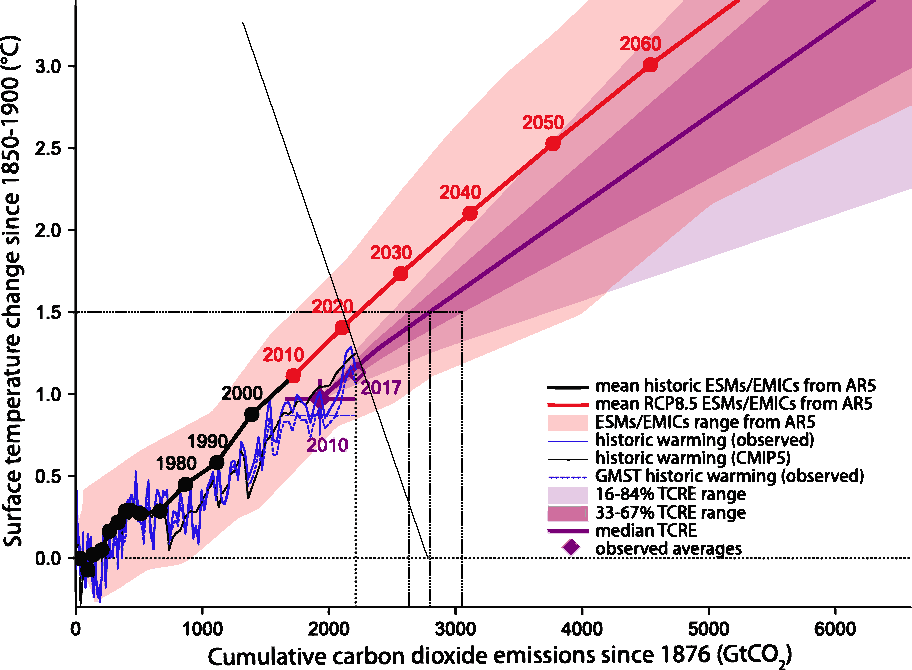
\includegraphics[width=0.9\linewidth]{bilder/cumulative_co2/cumulative_co2-4.pdf}
    \end{columns}

	\note{
	\begin{itemize}
		\item[] 
	\end{itemize}
	}
\end{frame}
